\documentclass[letterpaper,twocolumn,10pt]{article}
\usepackage{usenix,epsfig,endnotes}
\usepackage{algorithm}
\usepackage{algpseudocode}
\usepackage{amsmath}
\usepackage{amssymb}
\usepackage{caption}
\usepackage{subcaption}

\begin{document}

%don't want date printed
\date{}

%make title bold and 14 pt font (Latex default is non-bold, 16 pt)
\title{\Large \bf Position Estimation of Tractor and UAVs in Smart Agriculture}

\author{
{\rm Riccardo Periotto}\\
KTH Royal Institute of Technology\\
{\rm Stockholm, Sweden}\\
periotto@kth.se
\and
{\rm Mattia Sartori}\\
KTH Royal Institute of Technology\\
{\rm Stockholm, Sweden}\\
msartori@kth.se
}

\maketitle

% Use the following at camera-ready time to suppress page numbers.
% Comment it out when you first submit the paper for review.
\thispagestyle{empty}

\subsection*{Abstract}
\textbf{This report illustrates the motivation and the implementation of the final project of the course “EL2320 Applied Estimation” at KTH - Royal Institute of Technology. The project primarily focuses on applying particle filters to estimate the position of a tractor and two drones while harvesting. The environment is completely simulated in 2D using MATLAB. The sensors adopted are GNSS for globally identifying the tractor position and UWB to identify the relative position of the vehicles. The measurements of the UWB sensors are completely simulated, while the GNSS ones were taken from a real dataset, together with the real position of the tractor when moving in a field. 
The scenario is oversimplified, but the project helped us better understand the contents of the course. We had to deal with the usage of multiple particle filters and with sensors that were different from those used in the course. Developing the report allowed us to organise what we did for the project and better understand the selective harvesting field, in which many robotic applications are now under development.}

\textbf{\textit{Keywords}---Smart Agriculture, Selective harvesting, Applied Estimation, Particles Filters}


\section{Introduction}
Smart agriculture, also known as precision agriculture or digital agriculture, refers to the usage of advanced technologies and techniques to improve the efficiency and productivity of agricultural operations. Its core element is the integration of various sensors, devices, and systems to gather and analyse data about the agricultural fields, as well as to control and optimise their management. Smart agriculture is transforming traditional farming into a more data-driven and sustainable industry, by
allowing for more precise and targeted application of inputs, reducing waste and environmental impacts, and improving crop yields and quality. 


Considering the systems designed for precision agriculture, robots, unmanned ground vehicles (UGV) and unmanned aerial vehicles (UAV) are becoming widespread. Some applications in which they are already present are harvesting, seedling, spraying pesticides, and weed detection. 
Among the advantages of using aerial vehicles such as drones in agriculture is their ability to reach areas that may be difficult or impossible for humans to access, such as steep slopes or dense vegetation. They can also operate faster than humans, resulting in more efficient and cost-effective operations. 
In the typical harvesting scenario, auxiliary robots collect ripe crops from the field and bring them to a container, often attached to a ground vehicle such as a tractor. This one moves along the field lane while the others make multiple trips between the field and the container carrying the collected crops.

One of the main challenges of autonomous harvesting is to ensure the achievement of the preset tasks and do that with precision. 
Some examples of the required tasks are navigation in complex environments, identification and selection of plants or fruits, and avoidance of the risk of damaging crops or missing some.
To improve the success of these tasks, it is fundamental that the entities involved know their relative position and the surrounding environment. To do that, they perform what is called position estimation. Over the years, position estimation has been tackled with many different algorithms and sensors. This project is focused on and simulates one of such scenarios.

% \subsection*{Contribution}
In this work, we developed and tested particle filters for estimating the position of a tractor and two drones during crop harvesting in a 2D MATLAB simulation. The project development started from the code and user interface of the two laboratories of the "EL2320 Applied Estimation" course at KTH - Royal Institute of Technology. 
In the simulation, the tractor moves along a field lane with apples on both sides. The objective of the drones is to locate the apples, approach them, and carry them back to the tractor container. The particle filters estimate the 2D position of the tractor and the drones based on their motion model and the measurements they receive. We took the tractor position and the GNSS measurements related to it from a dataset generated from a real-world application and appropriately manipulated it for our project. The positions and measurements for the drones instead were completely generated from code.
The study focused on understanding the behaviour of the particle filters in the described scenario and on simulating sensors different from those studied in the course. Another aspect of the project different from the content of the course assignments is that there is no need for data association to match the measurements to the landmarks, as the only landmarks involved are the UWB antennas placed on the tractor. In this case, however, these landmarks are moving, causing their position to be uncertain. 
The drones are controlled by defining their directions and velocities. These are calculated using the ground truth information of the simulation. The project took inspiration from an application developed by an Israeli company called Tevel. The link in the footnotes points to a video showing how the system works in a real case \footnote{\url{https://www.youtube.com/watch?v=E0zGlWHYV3Q}}. The project code is available on GitHub \footnote{\url{https://github.com/riccardoperiotto/KTH_EL2320_AppliedEstimation}}. 

% \subsection*{Outline}
This report is structured as follows. \autoref{sec:2} describes the adoption of applied estimation in crop harvesting and presents an overview of the related literature. \autoref{sec:3} presents the main aspects of the tools involved in the project, together with an explanation of how we implemented them. \autoref{sec:4} illustrates the collected results, while the last section concludes the report with an analysis of the results and the field of study in general.

\section{Related work}
\label{sec:2}

\subsection*{Selective harvesting with drones}
Smart agriculture is a growing field that involves a wide range of techniques and technologies intending to improve the efficiency and sustainability of agricultural operations. These operations include harvesting crops, detecting and controlling weeds \cite{Gondchawar2016IoTBS}, managing water resources, applying fertilisers \cite{Gondchawar2016IoTBS, GonzlezDeSantos2017FleetsOR} and other inputs in a targeted and precise manner, and sowing \cite{7793638}, among others. In \cite{9374808}, the authors present a detailed review of emerging technologies for smart agriculture. In this study, we focused on the problem of harvesting, which involves collecting ripe crops from the field and transporting them to storage or processing facilities. There are two main types of harvesting: selective harvesting, in which only specific crops are picked, and mass harvesting, in which all crops in a certain area are collected \cite{e47335bdec694548b75225d317700e43}.

Selective harvesting of high-value crops, such as apples, tomatoes, and citrus,  is labour-intensive, making it an expensive task. Different sources indicate that harvesting can account for more than 25\% of the total cost for this kind of crop \cite{DutchCost, CostOrange}. 
To reduce this cost, researchers have been working on developing robotic systems for selective harvesting. These systems use various technologies, such as sensors, computer vision, and robotics, to identify and pick ripe fruits and vegetables while leaving unripe ones on the plant. 
According to van Henten \cite{RobotInHarvesting}, there have been numerous efforts over the past three decades to develop robots for automated harvesting, and the large number of proposed solutions in the literature on this topic indicates the same. However, multiple studies underline the presence of a gap between what is reported in the literature and what is used in commercial applications.
For example, in \cite{e47335bdec694548b75225d317700e43} they analysed the state-of-the-art solutions for harvesting and realised that only a couple of the considered solutions are currently in commercial use.
A similar result is the one presented in \cite{robotics10020052}, a research in which the authors performed a systematic review of agricultural robotic systems applied in land preparation, planting, sowing, plant treatment, harvesting and yield estimation. In their conclusion, they state that 80.65\% of the examined solutions are still in the research and development stage. These results suggest that, while there are many pre-commercial research and development initiatives for agricultural robotics, the technology is not yet fully developed and commercially viable. Despite numerous studies on various aspects of harvesting with robots, their performance is not yet sufficient to compete with human harvesters, probably due to the complexity of the task and the challenges of adapting the technology for practical use \cite{e47335bdec694548b75225d317700e43}.

In any case, research is going on and while the proposed applications of generic robotic systems for agriculture have been around for many years, solutions using drones are relatively new. Drones are gaining attention due to their ability to acquire field data in an easy, fast and cost-effective way compared to previous methods \cite{info10110349}. 
To the best of our knowledge, in most examples, UAVs are mainly used for 3D reconstruction, yield estimation, monitoring and spraying \cite{HAFEEZ2022, 9316211}.
A documented example similar to the scenario we simulate is \cite{GroundAndAerial}. In it, the researchers describe an application where a drone and a ground robot work together to monitor a field and apply selective spraying without human intervention. This example illustrates the potential of aerial and ground robots in agricultural applications, but it does not refer to harvesting.

The idea of using drones for harvesting comes from a system developed by Tevel, an Israeli company that has recently gained funding from investors and received media attention. On its website \footnote{\url{https://www.tevel-tech.com/}}, Tevel states that its system is designed for picking apples, peaches, apricots, nectarines, plums and pears. Honestly, it is now unclear to us at what stage of development the company's technology is, but we believed this to be out of the scope of the project, as we just considered the idea from the position estimation point of view.

\subsection*{Localization}
In the field of harvesting, several tasks need to be addressed. In this study and project simulation, we assume to have at our disposal methods to solve most of them. This is a legitimate assumption since we verified that the literature includes several methods for dealing with all the tasks the system needs. A non-exhaustive list of these tasks contains fruit detection \cite{BARTH2018284}, grasping with the correct end-effector \cite{agriculture12081240}, tractor navigation \cite{Stentz2002} and drones autonomous navigation \cite{DronesNavigation}. This study focused on position estimation, which in our simplified environment, corresponds to the process of determining the 2D location of the different vehicles while they are moving for harvesting. 

Sensor fusion and estimation algorithms improve the accuracy and reliability of the position estimate by combining data from multiple sensors and sources. Kalman and particle filters are two estimation algorithms used to perform sensor fusion. The book we took as a reference during the course explains these algorithms extensively \cite{thrun2005probabilistic}. In short, they are both algorithms that estimate the state of a system based on a system model and a sequence of noisy measurements. 
Kalman filters are considered optimal in the sense that they minimize the mean squared error of the estimate, but they assume a Gaussian system and measurement noises and a linear state transition model. Extended Kalman filters soften these assumptions, dealing with non-linear motion models. On the other hand, the particle filter represents the system's state as a set of discrete particles, each corresponding to a possible state of the system. In every iteration, it propagates the particles through time using a motion model, which represents the expected behaviour of the system. Sensor measurements are then used to select which particles to maintain and which ones to discard. The probability distribution over the system state is approximated, in each timestep, by the set of particles.

The choice of which algorithm to use depends on the specific characteristics of the system and the sensor data, such as the nature of the noise, the complexity of the motion model, and the required computational resources. We decided to use particle filters because, as explained in the book \cite{thrun2005probabilistic}, particle filters are particularly effective for position estimation in non-linear and non-Gaussian environments, such as those often encountered in agriculture. The position of the harvesting machinery may indeed be affected by external factors such as terrain, weather, and obstacles. These external factors can introduce uncertainty and variability into the position of the tractor and drones, which can cause the relative distribution to deviate from a Gaussian shape. In addition, they allow modelling non-linear constraints such as irregularities in the ground, fences or physical obstacles in a generally easier way than Kalman filters. In \cite{BLOK2019261}, researchers demonstrated how the adoption of particle filters for robot tracking in agriculture outperformed the usage of the Kalman one.

As anticipated, a peculiarity that all the bayesian filters have in common is the usage of the information provided by sensor measurements. In this work, we simulated the adoption of GNSS (Global Navigation Satellite System) and Ultra-wideband (UWB) technologies. GNSS measurements allow the filter to improve the global position of the tractor, while UWB technology calculates the relative position between the tractor and the drones.

GNSS (Global Navigation Satellite System) is a widely used technology for localisation. GNSS systems, such as GPS, GLONASS, and Galileo, use a network of satellites orbiting the Earth to transmit signals to receivers on the ground. By receiving and analysing these signals, GNSS receivers can determine their location with high accuracy \cite{Guo2018}. 

Ultra Wideband (UWB) technology is a wireless technology that uses radio waves to transmit data over a short distance. The DW1000 integrated chip (IC) is a transceiver designed to operate in the UWB frequency band used in many applications that require wireless communication and ranging. 
Some features of the DW1000 include low power consumption, high sensitivity, and more robustness in the presence of multipath to other wireless technologies (such as narrowband systems) \cite{8250079}. These characteristics are common to other UWB chips and allow them to operate with high accuracy for extended periods without recharging, making the technology perfectly suitable and reliable for the position estimation task we are considering.

\section{Applied estimation}
\label{sec:3}

\subsection*{Particle filter}
The book defines the particle filter as a recursive non-parametric algorithm, in the sense that it does not represent the distribution it adopts with a fixed functional form. As explained during the course, this is not the best name, as all the particles act exactly as parameters. A better name could be distribution-free filter, in the sense that there are no assumptions on the functional form of the underlying probability distribution \cite{AppliedEstimation}.

In chapter 4 of the book \cite{thrun2005probabilistic}, the authors thoroughly describe the filter and how to derive it mathematically. This document reports the most basic variant of the algorithm, as its steps are at the base of the code developed for the project. 

The particle filters approximate the distribution function over the state at time $t$ by a set of particles $\mathcal{X}_t=\{x_t^{[1]},\dots x_t^{[M]}\}$, where each particle represents a possible state in which the system can be. In the notation adopted in the course and the book, this function is called belief $bel(x_t)$, or posterior distribution over the state. The likelihood for a state hypothesis $x_t$ to be in the particle set $\mathcal{X}_t$ shall be proportional to the value of the posterior function. Ideally, the more samples from the set in a specific subregion of the state space, the more likely it is that the true state of the system falls into that region.


\begin{algorithm}
\caption{Algorithm Particle\_filter($\mathcal{X}_{t-1}$, $u_t$, $z_t$)}\label{alg:1}
\begin{algorithmic}[1]
\State $\bar{\mathcal{X}}_t \gets \mathcal{X}_t \gets \emptyset$
\While{$m \leq M$} 
    \State sample $x_t^{[m]} \sim p(x_t|u_t,x_{t-1}^{[m]})$
    \State $w_t^{[m]} \gets p(z_t|x_t^{[m]})$
    \State $\bar{\mathcal{X}}_t \gets \bar{\mathcal{X}}_t+<x_t^{[m]},w_t^{[m]}>$
\EndWhile
\While{$m \leq M$} 
    \State draw $i$ with probability $\propto w_t^{[i]}$
    \State add $x_t^{[i]}$ to $\mathcal{X}_t$
\EndWhile
\State return $\mathcal{X}_t$
\end{algorithmic}
\end{algorithm}

The pseudo-code of the particle filter algorithm is reported in Alg. \autoref{alg:1}.
The algorithm starts from an initial state set using any available information. Otherwise, it spreads the particles on the entire state in which the vehicle could be. In each iteration, the system's state is predicted based on the motion model and the control input provided at the specific time step. The filter compares its prediction with the observations and assigns a weight to each particle. The particles are then resampled, with more heavily weighted particles being more likely to be selected. As described in the book, this step can be performed in multiple ways \cite{thrun2005probabilistic}. In our project, one can decide whether to follow the multinomial or systematic approach.  The new particle set after the resampling describes the new approximation for the system state distribution.

To better organise the code, we developed a single class implementing the particle filter and instantiated an object for each tracked vehicle. We could have used a single filter working with the entire nine-dimensional system state, but we preferred to split the concepts and work with smaller, simpler matrices. The whole algorithm gets executed by calling a single function, which takes the current estimated state and measurement and returns a new state estimation and a boolean indicating whether the measurement is an outlier. 

\subsection*{Motion model}
Of fundamental importance for the simulation and the filter are the motion models of the entities involved. In a planar environment like the one considered here, the variables of such models are the $x$ and $y$ coordinates and the vehicle attitude $\theta$. In each iteration, the spatial coordinates are updated using a simplified unicycle motion model of an object moving towards a direction with a given velocity. Mathematically, the model equations are the following:

\begin{align*}
& x_t = x_{t-1}+v_t\times cos(\theta_{t-1})\times \Delta t\\
& y_t = y_{t-1}+v_t\times sin(\theta_{t-1})\times \Delta t\\
\end{align*}

The simplification derives from the fact that the vehicles' attitudes are defined deterministically according to the data and the control module, so there is no need to update it through the angular velocity as it would be necessary for the standard unicycle model.

The above model is used both in the prediction phase of the particle filter and to update the ground truth position of the drones. In both cases, we add Gaussian noise to the calculation.
The noise added in the prediction step is proportional to the motion noise matrices editable from the user interface. Its objective is to account for any errors or uncertainty in the predictions of the system state.  
The role of the second noise instead is to make the study more realistic and to check how the filter accounts for it.

\subsection*{Observation model}
The main difference between running the particle filter for the tractor and running it for the drones stands in the observation model.
The observation model of a particle filter is used to predict the observation value given the state estimation. In our case,  we have a model that returns the estimated global position for the tractor and another that retrieves the estimated relative position to the tractor for drones. A measurement is labelled as an outlier when the difference between it and the value returned by the observation model is significant. The comparison is not performed directly on the measurement, but instead, a likelihood value is calculated by averaging the Mahalanobis distance between the expected measurement considering all the particle states and the one observed. If this average is below a fixed threshold, then the measurement is labelled as an outlier. This approach is the same followed in the two laboratories.

The percentage of outliers generated for the UWB can be modified through the interface. The number shown on the interface, however, does not correspond to the number of outliers the system will have at the end of one simulation execution, as the observation model used by the drones adopts the estimated position of the tractor, which is itself uncertain. 

Concerning the tractor, there is not much to change in terms of measurements and outliers, as they mainly depend on the imported real data. The only adjustable parameters are the noise matrix elements and the likelihood threshold.

\subsection*{Ultra Wideband (UWB)}
The previous section already provided some advantages of UWB technology.
This section illustrates how to calculate the relative position of devices using UWB messages. As anticipated, the UWB protocol directly provides the range between two devices obtained, for example, by multiplying the signal Time of Flight (ToF) by the speed of light.
Representing the relative position of one point to another on a plane, on the other hand, is a less trivial operation. We encountered at least two ways of doing this: the first via a range and an angle, the second via the relative Cartesian coordinates $x$ and $y$. Both cases require a second antenna at a known distance $d$ from the first. 
\cite{8250079} follows the first way and presents different possible calculations for the angle of arrival (AOA). 
In the project, we simulate the usage of the second method, patented and described in \cite{patent}. The novelty here is that the range and path difference are used directly for calculating the relative coordinates, without going through intermediary steps for calculating the angle. The path difference $p$ is the difference between the distance from the transceiver to the first antenna and the second.  $p$ can be calculated using the difference in the phase, the difference in time of arrivals or the difference in ranges, with the first method being the most accurate  \cite{patent}.
Assuming that $d$ is less than half the wavelength $\lambda$, the formulas for calculating $x$ and $y$ are the following:

\noindent
\begin{align*}
& cos(\alpha)=(r^2 + d^2 - (r-p)^2)/2rd \\ 
& x/r = (r^2+d^2-r^2+2rp-p^2)/2rd \\
& p = r - r_2 \\
& x = (d^2+2rp-p^2)/2d \\
& y = \sqrt{r^2-x^2}
\end{align*}

We reported the first two equations to show how to apply Carnot's theorem. The third equation is used in the simulation to calculate $p$. In an integrated circuit, this calculation would be substituted by one of the methods described in the patent. $r$ and $r_2$ are the ranges measured between the transceiver and the two receiver antennas.
The geometric representation from which the presented calculations derive is in \autoref{fig:1}.

\begin{figure}[!htp]
    \centering
     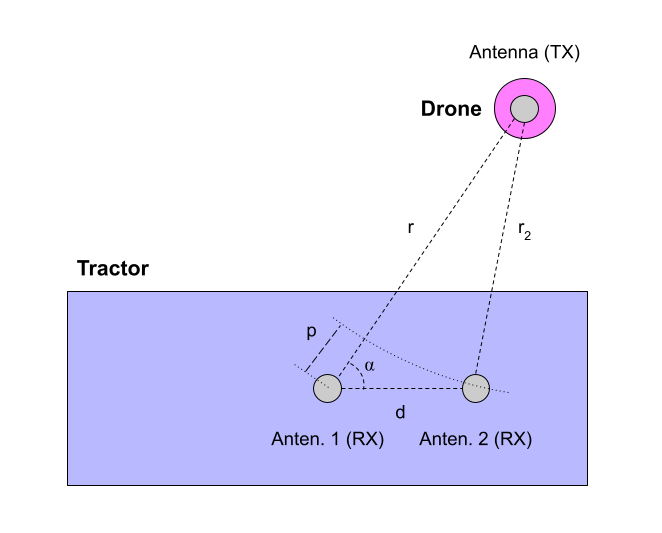
\includegraphics[width=8cm]{images/uwb.png}
     \caption{\textbf{UWB relative position calculation.} The schema illustrates the different distances used to calculate the relative position of the drone to the tractor. The geometry followed by the layout is the same as that described in the patent \cite{patent}.}
    \label{fig:1}
\end{figure}

The square root gives two completely equivalent solutions, differing only in the sign of $y$. The simulation solves the problem by assuming that each drone is always on one side of the tractor. 
In the simulation, we assumed to use the Decawave DW1000 IC, which carrier frequency is $6.5 GHz$. The value for the parameter $d$ is then:
\begin{align*}
& d = \frac{\lambda}{2} = \frac{1}{2} \times \frac{c}{f} \sim 0.022 m
\end{align*}

We also assumed that the first antenna in the middle of the tractor. This assumption can be softened by using roto-translation matrices to compensate for any fixed shifts.


\subsection*{Global Navigation Satellite System (GNSS)}

As anticipated, the tractor particle filter uses GNSS measurements in its update phase. We could not conduct real experiments to test the algorithm, but differently from the case of tracking drones, we took both the position and the measurements from a real dataset. The dataset comprises approximately 2 hours of sensor data from a tractor-mounted sensor system in a grass-mowing scenario \cite{s17112579}.
The amount of data collected is vast, including images from different types of cameras, LiDAR and radar, IMU and GNSS,
but we just took the last one. In addition to the raw sensors data, the project also shares a sequence of global positions obtained by the fusion of IMU and GNSS by the  EKF developed in \cite{10.1007/978-3-319-08338-4_25}. We took a part of this sequence as the tractor ground truth of our studies.

The GNSS measurements come from a Trimble BD982 GNSS, a dual RTK antenna working at 20 Hz \cite{trimble}.  
RTK (Real-Time Kinematic) GNSS is a precise positioning technique used to determine the real-time location of a receiver starting from GNSS measurements. It works thanks to a reference station which receives the same signals as the receiver and employs its known location to calculate the errors in the satellite signals. These errors are transmitted to the receiver, which uses them to correct its position calculation up to an accuracy of a few centimetres or less \cite{wasoft}. 


The global geographical data in the dataset follows a GCS format. To use this data in our application, some transformations were necessary. 
For simplicity, we selected a data interval in which the tractor was moving in a straight direction for 30 seconds. We then converted the coordinates within this interval from GCS to UTM (Universal Transverse Mercator) coordinate system thanks to the utm Python library \footnote{\url{https://pypi.org/project/utm/}}. The final step was to shift and rotate the data to align the first point of the interval to the simulation starting point and the direction along which the tractor moves to the layout x-axis.

The average tractor speed derived from the ground truth data is $1.43 m/s$. This speed could be excessive or not for harvesting depending on how many fruits are present in the field lane. We kept it as it comes after noticing that in our simulation, with a low density of apples, it worked fine. In any case, speed can always be scaled by simulating different intervals between data samples.

\subsection*{Control}
As underlined multiple times, the project's focus was the application of estimation algorithms. However, as the vehicles had to move according to specific target tasks, a minimum part of control was necessary.

Because of how we transformed the real data, the tractor's attitude is always zero, and its speed remains constant throughout the simulation. On the other hand, the direction and speed of the drones are computed in each iteration according to their position and the task they have to perform. 
 
While the drone does not detect apples, its goal is to stay at a fixed distance from the tractor. When an apple is individuated, drone speed increases and its direction changes pointing towards the fruit. In the simulation, the drone never misses an apple it is tracking and can always pick it up once it reaches it.
The drone's direction is then recalculated at each iteration until it gets back to the tractor and releases the apple. From there, the drone restarts its detecting phase from scratch.

\begin{figure}[!htp]
    \centering
     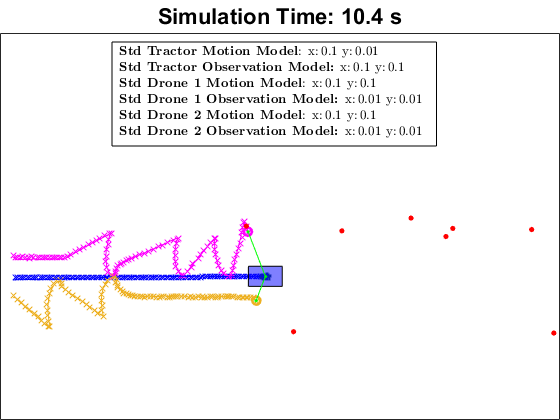
\includegraphics[width=7.5cm]{images/screenshot_example.png}
     \caption{\textbf{Simulation screenshot.} The cyan rectangle is the tractor, while the two circles are the drones. The three solid lines are the ground truth of the three vehicles, while the 'X's indicate the estimated position at each timestep. The estimation is given by the average of the particles, which are visible only for the tractor because those of the drones are covered by their edges. The seven red dots spread on the right of the tractor are the apples. The first drone is carrying an apple toward the tractor, while the second just detected an apple after moving at its offset distance from the tractor for a few metres. The lines connecting the drones to the tractor represent the UWB measurements. The single dot in the middle of the tractor is the GPS measurement. In this case, all the measurements are in green, meaning there are no outliers.  }
    \label{fig:2}
\end{figure}

\subsection*{Simulation sample}
Now that we explained all the main parts of the project from the theoretical point of view and concerning our implementation, we can report a screenshot taken from the running simulation (\autoref{fig:2}). The noises and outliers parameters set for launching the simulation are currently not fundamental, as the only purpose of this subsection is to allow the reader to visualise what we did and better comprehend the following section. In all the experiments considered for this document, the three filters have 1000 particles each. Also, the number and position of the apples follow always the same standard displacement. By doing this, we could compare the performances of the filters in different executions only according to the parameter values, and not depending on the tracks followed by the vehicles. To entirely avoid randomness, we also run the simulation assuming to receive a GNSS measurement every five iterations. In the code published, this feature is modelled with a 20\% probability of measurement occurrence in each iteration. 

Unless otherwise specified, the simulation adopts multinomial resampling and outlier detection is active. The threshold for outlier identification is 2, as in the laboratory default.

\section{Experiments and results}
\label{sec:4}
To understand the goodness of the particle filter, we studied its behaviour in various situations. Estimation and uncertainties usually play the role of the highest importance in these moments, since they represent exactly how well the filter performs the task it is designed for. In our simplified scenario, other aspects prove more interesting to analyse, always considering errors and uncertainties as metrics.

\subsection*{Importance of GNSS}
For the simulated scenario, it is of utmost importance to know precisely where the tractor is located within the field, even because the drones only orient themselves with their position relative to it. In this section, we report the study of the system behaviour without GNSS updates when the tractor filter only performs the prediction step. 

The first trivial result is that no matter how we set the noise parameters, the uncertainty for the estimated tractor position will always increase. With a standard deviation of $0.05m$ on each motion and measurement model, the uncertainties behave as shown in \autoref{fig:3}. The aspect to note is that, given the frequent and precise UWB measurements, the uncertainties of the drone filters remain small, even though the estimated position may be wrong.

By doubling the standard deviations to $0.1$ in the code we initially wrote, also the uncertainty of the drone filters exploded at some point. This occurred because the filter decides whether or not to perform the update step with the UWB measurement based on the uncertainty of the tractor position. The filter uses the latter in the observation model, but it does not make sense to perform the update step when it is too high. Verifying this condition also allows us to apply the filter directly for the global estimation problem, where the tractor position is initially unknown.
Without the check, the drones will use the first UWB measurement to locate themself relatively to the given estimated position of the tractor, which falls in the middle of the field, obtained by averaging the tractor particles homogeneously spread throughout the field lane. The first few times we ran the simulation, the threshold on the standard deviation of tractor uncertainty within which to consider the UWB measurements was one meter and reached the 101st iteration. From there, the uncertainty of the drone filters also increased throughout the rest of the run, as in the complete absence of UWB measurements. \autoref{fig:4} and \autoref{fig:5} respectively show the uncertainty behaviour and its explosion in iteration 102. In the final version of the code, we set a threshold that ensures the avoidance of this behaviour, but to a value such that the algorithm works for global localization.

\begin{figure}[p]
    \centering
     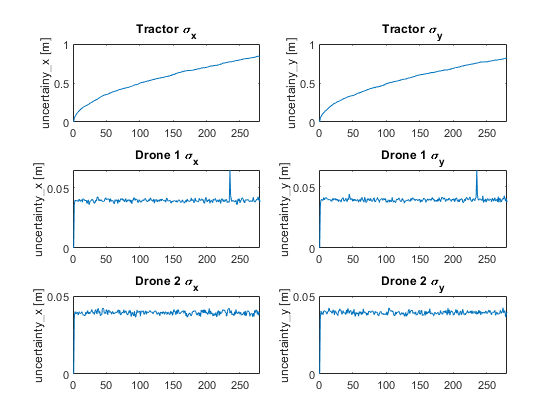
\includegraphics[width=7.5cm]{images/noGNSS_medium_noise_uncertainties.png}
     \caption{\textbf{Increasing tractor uncertainty.} The tractor uncertainty increments throughout the simulation, while that of the drones remains low in this first case. }
    \label{fig:3}
\end{figure}

\begin{figure}[p]
    \centering
     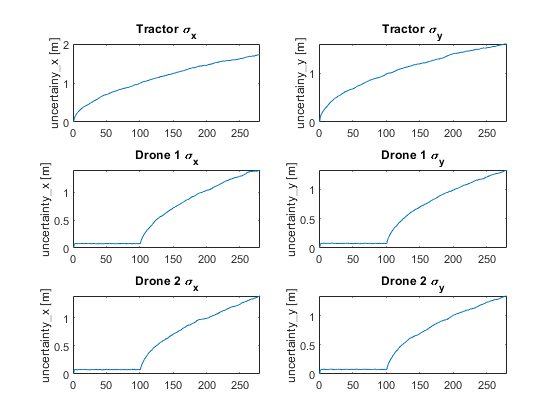
\includegraphics[width=8cm]{images/noGNSS_high_noise_uncertainties.png}
     \caption{\textbf{Increasing system uncertainty.} If the uncertainty on the tractor exceeds the coded threshold, UWB measurements are discarded and the uncertainty of drones increases.}
    \label{fig:4}
\end{figure}

\begin{figure}[p]
     \centering
     \begin{subfigure}[b]{0.23\textwidth}
         \centering
         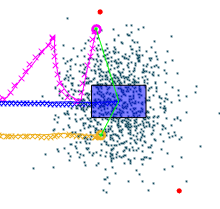
\includegraphics[width=\textwidth]{images/no_GNS_high_noise_101_touse.png}
         \caption{Iteration 101}
         \label{fig:5a}
     \end{subfigure}
     \hfill
     \begin{subfigure}[b]{0.23\textwidth}
         \centering
         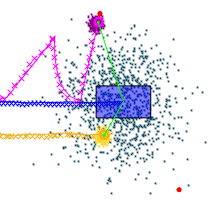
\includegraphics[width=\textwidth]{images/no_GNS_high_noise_102_touse.png}
         \caption{Iteration 102}
         \label{fig:5b}
     \end{subfigure}
     \caption{\textbf{Particles explosion.} Explosion of the drones particles when starting to discard UWB measurements in iteration 101 because of tractor position uncertainty over the threshold. }
     \label{fig:5}
\end{figure}


\subsection*{Outliers detection}
Outliers detection avoids updating the filter with misleading information. However, the incorrect combination of thresholds and noise matrices can make the outliers identification step erroneous.
For example, with a standard deviation of $0.01m$ on each motion and measurement model, the algorithm identifies 143 outliers out of 614 measurements. We know that, in the simulation, measurements are never outliers, unless set through the interface. The situation improves with a standard deviation of $0.05$, where no measurements are classified as an outlier. 

For the reader unfamiliar with particle filters, this result may be weird, since the meaning is that by increasing the noise of the models we obtain better results. The reason behind the observed behaviour is that, with higher noise, the distribution of particles dilates and the tolerance on a measurement error increases, allowing the filter to be less strict in considering the measurements. One should not take advantage of this by increasing model noises dramatically, because this would lead to a collapse in performance. Like in many other situations, the best solution is a trade-off.

As anticipated, the estimation error is not that meaningful in our simulation and remains almost unchanged regardless of the number of outliers. The error in the previous two cases is essentially the same, as well as that obtained when we force 50\% of the measurements to be outliers. This is also thanks to the algorithm for identifying outliers, which proved its effectiveness. Without it, the estimation error would be much higher, as shown in \autoref{fig:6}.

\begin{figure}[!h]
     \centering
     \begin{subfigure}[b]{0.23\textwidth}
         \centering
         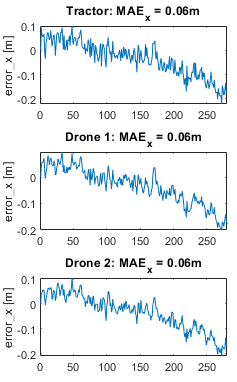
\includegraphics[width=\textwidth]{images/medium_noise_outlier_detection_touse.png}
         \caption{50\% outliers with detection}
         \label{fig:6a}
     \end{subfigure}
     \hfill
     \begin{subfigure}[b]{0.23\textwidth}
         \centering
         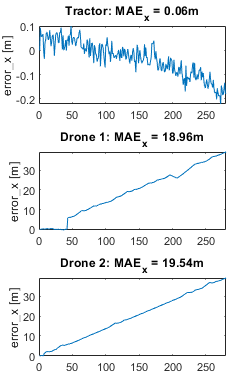
\includegraphics[width=\textwidth]{images/medium_noise_outlier_nodetection_touse.png}
         \caption{50\% outliers no detection}
         \label{fig:6b}
     \end{subfigure}
      \caption{\textbf{Outlier detection.} Error estimation when adding 50\% of outliers and applying or not the detection procedure. Only the behaviour along the x-axis is reported, but along the y-axis, the behaviour is the same. }
     \label{fig:6}
\end{figure}

Different is the case of uncertainty, which increases with both the standard deviation and the number of outliers, as shown in \autoref{fig:8}.


\subsection*{Global localization}
We tested the code for solving the global localization problem, confirming the effectiveness of the particle filter. The particles move according to the motion model until the first GNSS measurement arrives, with which the tractor can geolocate itself. Unlike in some scenarios in the second laboratory, in this case, the update does not suffer from multiple hypotheses, since there are no landmarks symmetries. When the uncertainty on the tractor's position becomes acceptable, the drones also make the update step with the UWB measurements and the observation model. By doing so, their uncertainty also drops dramatically. Everything happens in a single iteration, which in the case under consideration is the fifth. \autoref{fig:9} shows the situation before and after the arrival of the GNSS measurement.

In the iteration in which global localisation occurs, the filters suffer from particle deprivation. As shown in \autoref{fig:9b}, practically none of the 3000 particles representing the positions of the three vehicles are visible (although there are some, as we will explain in a moment). 
The reason for this behaviour comes from what the particle filter section above explains. When a new measurement arrives, the filter calculates, for each particle, a weight proportional to its probability of representing the true state given the new information. 
By doing this, only a few particles for each filter received a significant weight and those are consequently also the only particles selected when proceeding with the resampling phases. \autoref{tab:1} shows these particles, together with the received measurement and the one estimated considering the particle state in the observation model. 
This phenomenon is called particle deprivation and can lead the algorithm to a completely degenerate solution. In this case, thanks to diffusion, it lasts only for one iteration, which we believe is acceptable, considering the improvement in position estimation that it brings. 

%\subsection*{Resampling comparison}
%The resampling mode does not affect the performance of the algorithm. Errors and uncertainties remain practically the same whether multinomial or systematic resampling is applied. This usually occurs when the probability is well distributed among the filter particles.

\subsection*{Localisation performance}
In many analysed scenarios, particle filters prove their ability to track the harvesting vehicles. Simulating with the standard deviation of the motion and measurement noises set to a few centimetres (i.e. $3-10cm$) always results in errors similar to those reported in \autoref{fig:7}. In the provided case, the average error is $6cm$ along $x$ and $2cm$ along $y$. The maximum error reaches $20cm$ in $x$, which is a bit too high for the scenario analysed.

\begin{figure}[!htp]
    \centering
     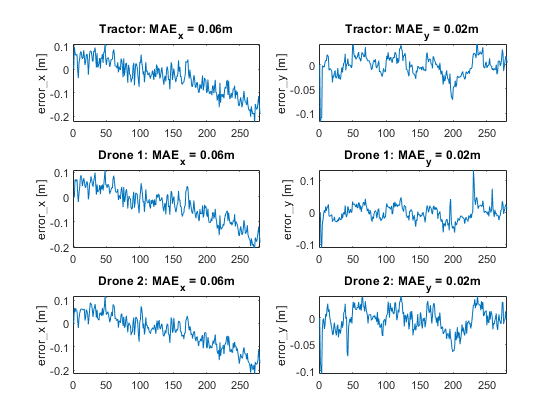
\includegraphics[width=8cm]{images/final_error.png}
     \caption{\textbf{Estimation error.} Typical behaviour of the errors when standard deviations are of a few centimetres.}
    \label{fig:7}
\end{figure}
The error pattern is similar for the various vehicles. This is probably because the system only relies on a single global measurement source. The drones receive their measurements relative to the tractor position, but cannot know how much this is correct to the absolute reference frame. If the GNSS measurements repeatedly have an offset, the tractor estimated position shifts accordingly. The particle filters tracking the drones can not identify this shift and move their estimated position in the same way.




\section{Discussion and conclusion}
We simulated the problem of localisation of vehicles for harvesting in a simplified 2D case using different sensors from those seen during the course.
The results obtained are good, but not excellent for our application. With an error of $20cm$, the risk of damaging the fruit, running into obstacles or hurting people is too high. 

Additional sensors, such as LiDAR, IMU or cameras, would help to increase performance. Cameras are required in any case for apple detection. Adding sensors would also make it possible to create a map of the environment, making the resolution of other tasks easier, navigation especially. This could be done, for example, by placing fixed reference points in the field or applying SLAM.

We have shown that the GNSS measurement alone can achieve remarkable results and solve the global localisation problem. However, an additional global measure would avoid the shift issue presented in the previous section.

Overall, the project allowed us to delve into the world of smart agriculture and understand how many aspects of this field are being automated worldwide, especially with robots and unmanned vehicles. We are looking forward to receiving new updates about the Tevel project. 

\begin{figure*}[!h]
     \centering
     \begin{subfigure}[b]{0.40\textwidth}
         \centering
         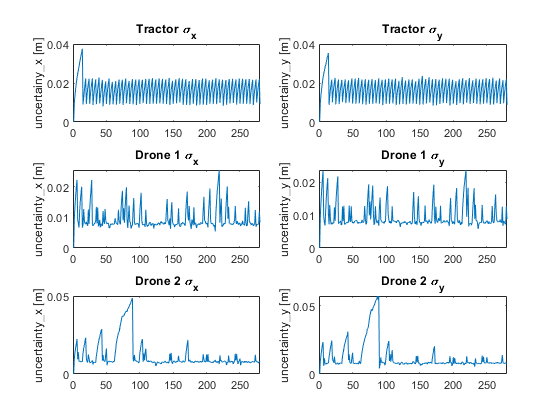
\includegraphics[width=\textwidth]{images/1.png}
         \caption{0.01m standard deviation.}
         \label{fig:8a}
     \end{subfigure}
     \hfill
     \begin{subfigure}[b]{0.40\textwidth}
         \centering
         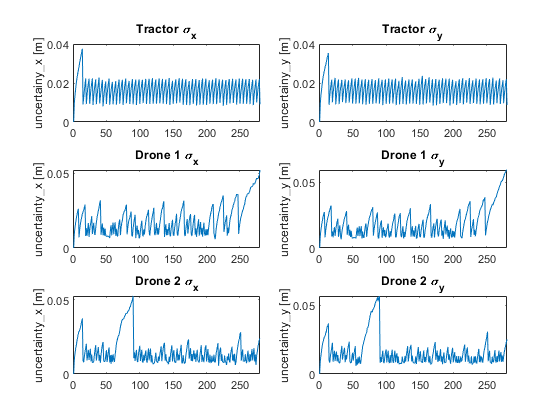
\includegraphics[width=\textwidth]{images/2.png}
         \caption{0.01m standard deviation and 50\% outliers.}
         \label{fig:8b}
     \end{subfigure}

    \begin{subfigure}[b]{0.40\textwidth}
         \centering
         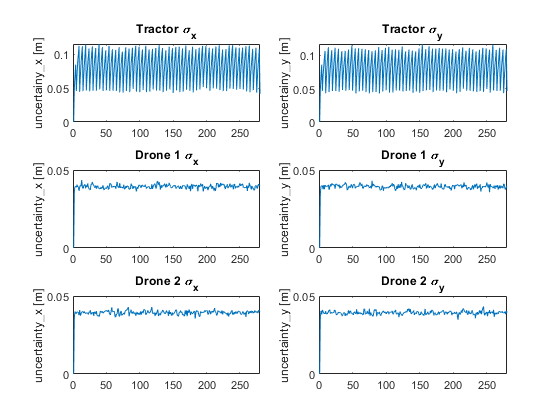
\includegraphics[width=\textwidth]{images/3.png}
         \caption{0.05m standard deviation.}
         \label{fig:8c}
     \end{subfigure}
     \hfill
     \begin{subfigure}[b]{0.40\textwidth}
         \centering
         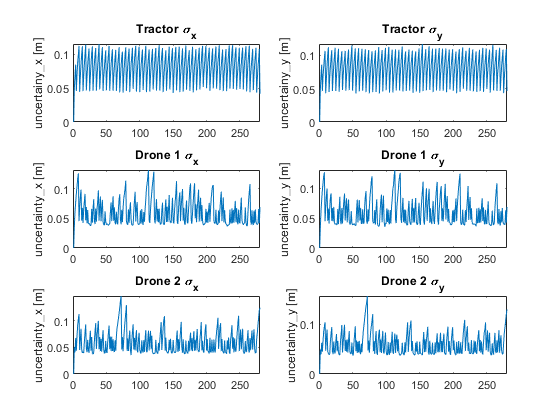
\includegraphics[width=\textwidth]{images/4.png}
         \caption{0.05m standard deviation and 50\% outliers.}
         \label{fig:8d}
     \end{subfigure}
     
     \caption{\textbf{Outliers and uncertainty.} The overall uncertainty increases with the number of outliers, as the update step is performed fewer times. As could be expected, also increasing the standard deviation of the models affects negatively the uncertainty. }
     \label{fig:8}
\end{figure*}


\begin{figure*}[!h]
\centering
     \begin{subfigure}[b]{0.40\textwidth}
         \centering
         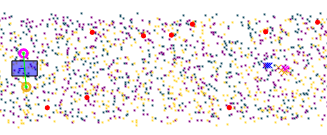
\includegraphics[width=\textwidth]{images/global_medium_noise_4_touse.png}
         \caption{Iteration 101}
         \label{fig:9a}
     \end{subfigure}
     \hfill
     \begin{subfigure}[b]{0.40\textwidth}
         \centering
         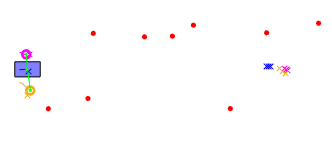
\includegraphics[width=\textwidth]{images/global_medium_noise_5_touse.png}
         \caption{Iteration 102}
         \label{fig:9b}
     \end{subfigure}
     \caption{\textbf{Global localization.} The two figures represent the situation before and after the arrival of the first GNSS measurement. }
     \label{fig:9}
\end{figure*}


\begin{table*}[htb!]
    \centering
    \begin{tabular}{ccccccc}\hline
    \textbf{Vehicle} 
    & \textbf{Real position}
    & \textbf{Measurement} $z$
    & \textbf{Particle index} 
    & \textbf{Particle coordinates}
    & \textbf{Predicted measurement} $\hat{z}$\\ \hline
    tractor & \ 0.6347, -0.0981 & \ 0.5751, -0.1007 & 220 & \ 0.6772, -0.2112 & 
    \ 0.6772, -0.2112 \\
            &                 &                 & 675 & 0.6297, 
    -0.2824 & \ 0.6297, -0.2824 \\
    \hline
    drone 1 & \ 0.5298, \ 0.8902 & -0.1131, \ 0.9919 & 972 & \ 0.7560, 
    \ 0.8782 & \ 0.0816, \ 1.0937 \\ 
    \hline
    drone 2 & \ 0.8479, -1.5018 & \ 0.2248, -1.3937 & 606 & \ 0.6207, 
    -1.8296 & -0.0536, -1.8296 \\          
    \end{tabular}
    \caption{\textbf{Particle deprivation.} Particles with more than a thousandth probability at the fifth iteration and related information. The probability of these particles practically corresponds to the total one; the one-thousandth threshold is purely symbolic. }
    \label{tab:1}

\end{table*}

{\footnotesize \bibliographystyle{acm}
\bibliography{sample}}


\end{document}







